%\documentclass[12pt]{article}
%\usepackage[a4paper, margin=1in]{geometry} 
%\usepackage{graphicx} 
%\usepackage{hyperref}
%\usepackage{float}
%\usepackage{multicol}
%\usepackage{multirow}
%\usepackage[font=small, labelfont=bf]{caption}
%\usepackage{amssymb}
%\usepackage{amsmath}
%
%\begin{document}

%
% Basic evaluation measures 
%
\subsection{Basic evaluation measures}
Various measures can be derived from the confusion matrix.

%
% Accuracy
%
\subsubsection*{Accuracy}

$\dfrac{TP+TN}{TP+FP+TN+FN} = \dfrac{TP+TN}{P+N} $
\begin{figure}[H]
  \centering
      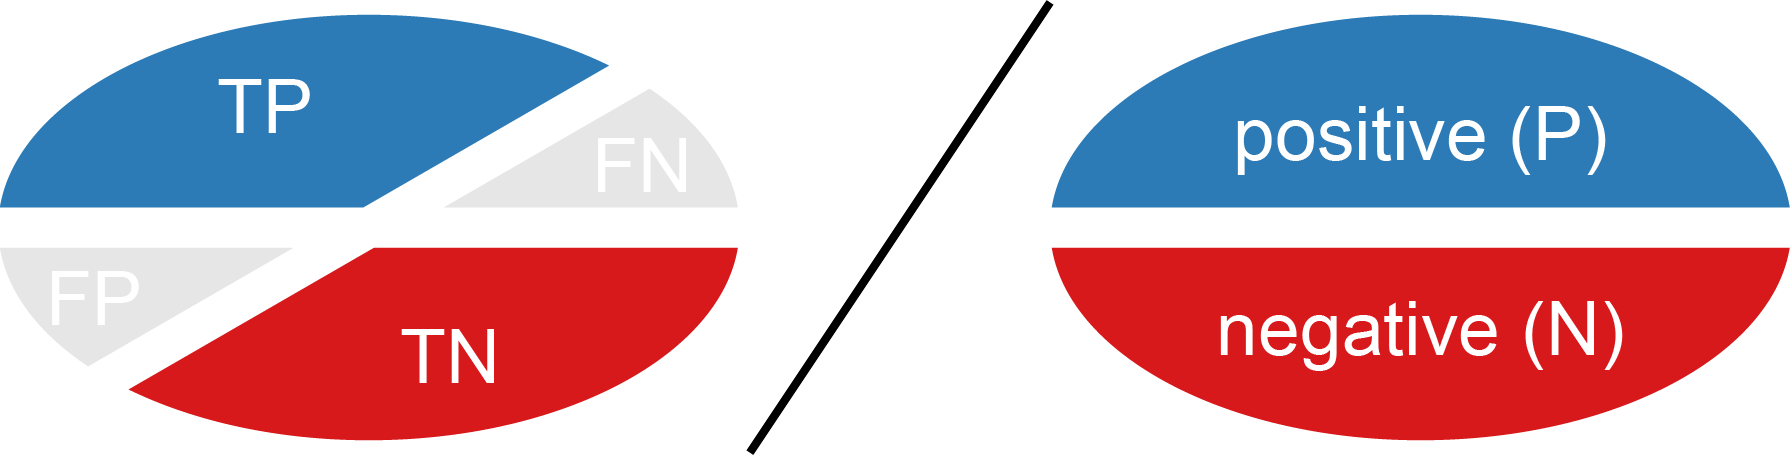
\includegraphics[width=0.4 \textwidth]{fig07/accuracy.png}
\end{figure}

%
% Error rate
%
\subsubsection*{Error rate}

$\dfrac{FP+FN}{TP+FP+TN+FN}= \dfrac{FP+FN}{P+N} $

\begin{figure}[H]
  \centering
      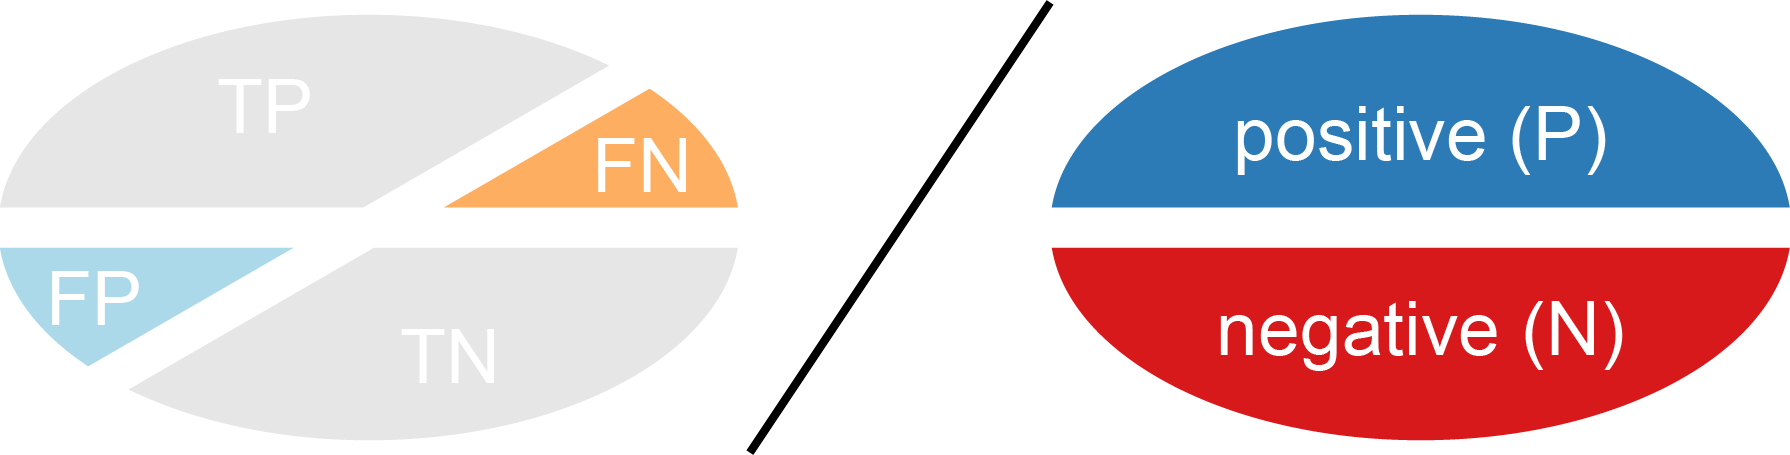
\includegraphics[width=0.4 \textwidth]{fig07/error-rate.png}
\end{figure}

%
% Sensitivity, True positive rate, Recall
%
\subsubsection*{Sensitivity, True positive rate, Recall}

$\dfrac{TP}{TP+FN}= \dfrac{TP}{P} $

\begin{figure}[H]
  \centering
      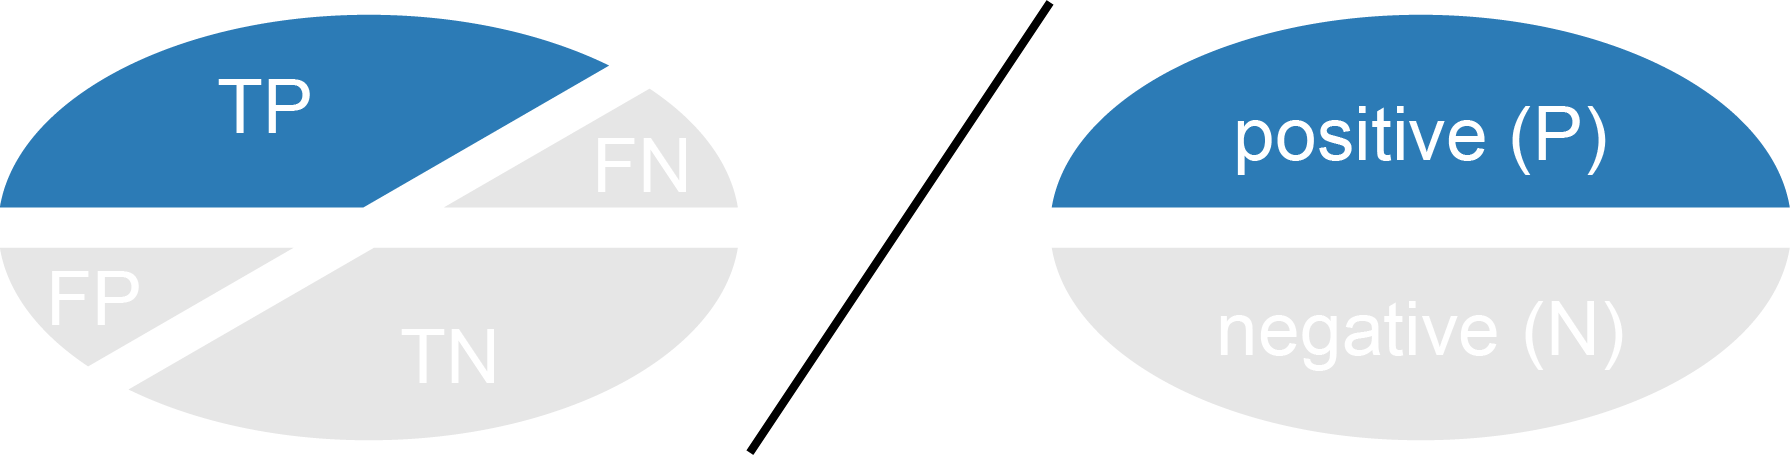
\includegraphics[width=0.4 \textwidth]{fig07/sensitivity.png}
\end{figure}

%
% Specificity, True negative rate
%
\subsubsection*{Specificity, True negative rate}

$\dfrac{TN}{FP+TN}= \dfrac{TN}{N} $

\begin{figure}[H]
  \centering
      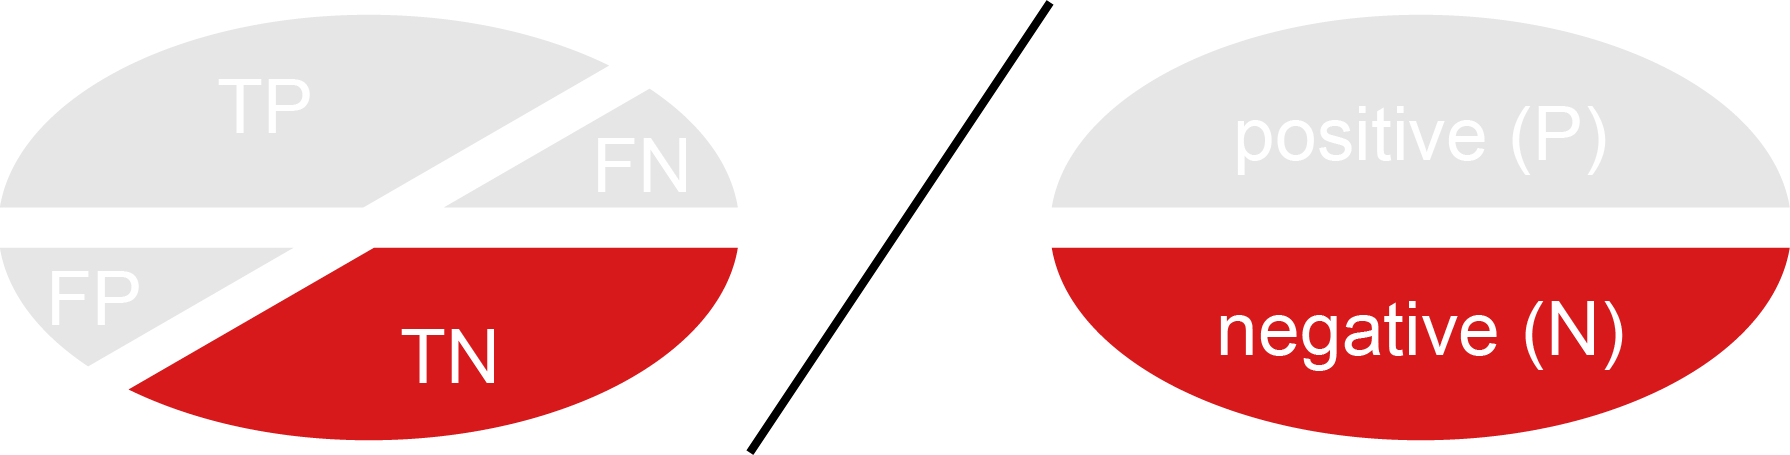
\includegraphics[width=0.4 \textwidth]{fig07/specificity.png}
\end{figure}

%
% Precision, Positive predictive value
%
\subsubsection*{Precision, Positive predictive value}

$\dfrac{TP}{TP+FP}$

\begin{figure}[H]
  \centering
      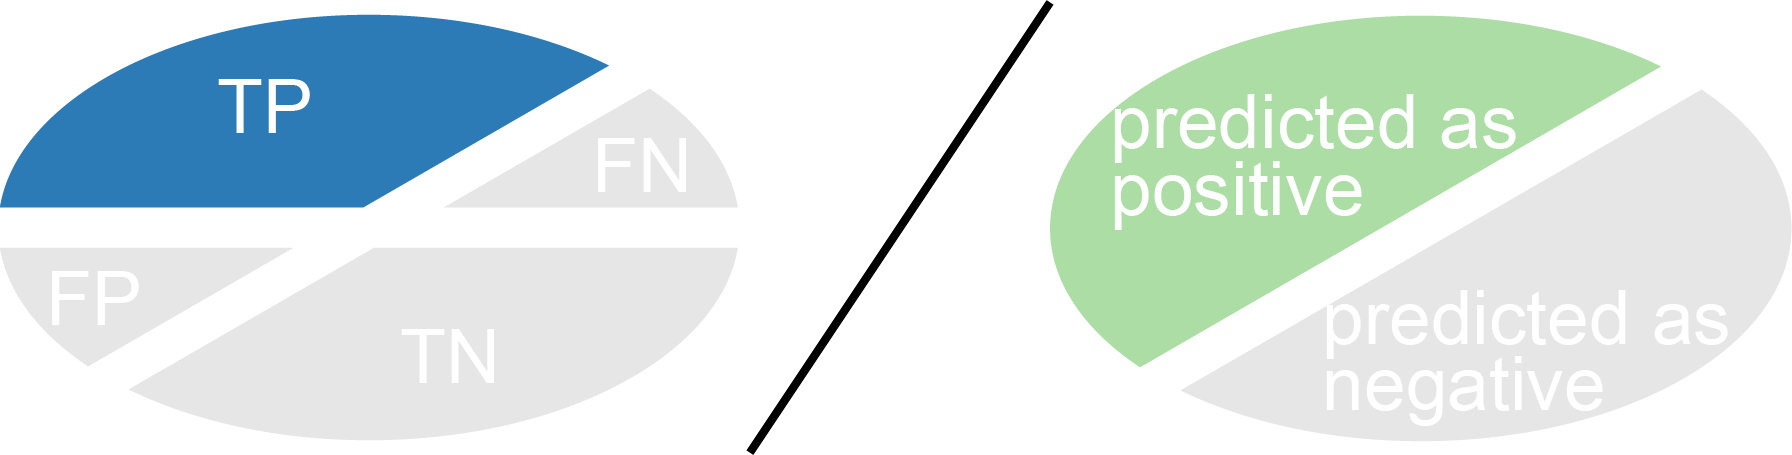
\includegraphics[width=0.4 \textwidth]{fig07/precision.png}
\end{figure}

\bigskip 

%\end{document}
